\documentclass[twoside,twocolumn,8pt]{extarticle}
\usepackage{subfigure}

% ------
% Fonts and typesetting settings
\usepackage{amsmath}
\usepackage{amssymb}
\usepackage[sc]{mathpazo}
\usepackage[T1]{fontenc}
\linespread{1.05} % Palatino needs more space between lines
\usepackage{microtype}


% ------
% Page layout
\usepackage[hmarginratio=1:1,top=10mm,columnsep=20pt,left=0.8in, right=0.8in]{geometry}
\usepackage[font=it]{caption}
\usepackage{paralist}
\usepackage{multicol}

% ------
% Lettrines
\usepackage{lettrine}


% ------
% Abstract
\usepackage{abstract}
	\renewcommand{\abstractnamefont}{\normalfont\bfseries}
	\renewcommand{\abstracttextfont}{\normalfont\itshape}


% ------
% Titling (section/subsection)
\usepackage{titlesec}
\renewcommand\thesection{\Roman{section}}
\titleformat{\section}[block]{\large\scshape\centering}{\thesection.}{1em}{}

\usepackage{graphicx}
% ------
% Header/footer


\usepackage{fancyhdr}
\pagestyle{fancy}

\setlength\headheight{90.0pt}
\addtolength{\textheight}{-90.0pt}

\fancypagestyle{firststyle}
{
   	\fancyhead[L]{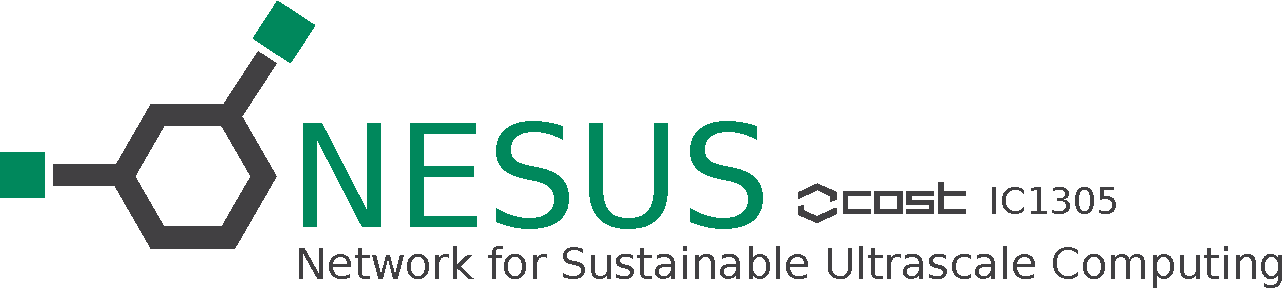
\includegraphics[height=5.5em]{pictures/nesus.pdf}}
	\fancyhead[C]{}
	\fancyfoot{}
	\fancyhead[R]{\small{Book paper template $\bullet$ October 2016 $\bullet$ Vol. I, No. 1}}
	\fancyfoot[RO,LE]{\thepage}
}
	\fancyhead[R]{}
	\fancyhead[L]{}
	\fancyfoot{}
	\fancyhead[C]{\small{Book paper template $\bullet$ October 2016 $\bullet$ Vol. I, No. 1}}
	\fancyfoot[RO,LE]{\thepage}


% ------
% Clickable URLs (optional)
\usepackage{hyperref}

% ------
% Maketitle metadata
\title{\vspace{-10mm}%
	\fontsize{24pt}{10pt}\selectfont
	\textbf{Automatic Cache Aware Roofline Model Building and Validation Using Topology Detection}
	}
	
		
\author{%
	\large
	\textsc{Nicolas Denoyelle \& Aleksandar Ilic \& Brice Goglin \& Leonel Sousa \& Emmanuel Jeannot} \\[2mm]
	\normalsize{	Inria - France -- INESC-ID -- Portugal}\\
	\normalsize{	\href{mailto:nicolas.denoyelle@inria.fr}{nicolas.denoyelle@inria.fr} \href{mailto:ilic@sips.inesc-id.pt}{ilic@sips.inesc-id.pt} \href{mailto:brice.goglin@inria.fr}{brice.goglin@inria.fr} \href{mailto:las@sips.inesc-id.pt}{las@sips.inesc-id.pt}} \href{mailto:emmanuel.jeannot@inria.fr}{emmanuel.jeannot@inria.fr}
	\vspace{-5mm}
	}

\date{}

\providecommand{\keywords}[1]{\textbf{\textit{Keywords}} #1}

%%%%%%%%%%%%%%%%%%%%%%%%
\begin{document}



\twocolumn[
  \begin{@twocolumnfalse}

\maketitle

\thispagestyle{firststyle}


\begin{abstract}
  \noindent The ever growing complexity of high performance computing systems imposes significant challenges to exploit as much as
  possible their computational and memory resources. Recently, the Cache-aware Roofline Model has gained popularity due to its
  simplicity when modeling multi-cores with complex memory hierarchy, characterizing applications bottlenecks, and quantifying
  achieved or remaining improvements. In this short paper we involve hwloc topology detection to build  the Cache Aware Roofline
  Model for modern processors in an open-source locality-aware tool. The results we obtained on platform benchmarking with the
  tool, reach near-theoretical bounds and show the model methodology effectiveness.
\end{abstract}


\keywords{Roofline Model, DRAM, Cache, Tool, Cache Aware Roofline Model, hwloc}

 \hrulefill
\bigskip 


\end{@twocolumnfalse}
]


\section{Introduction}\label{sec:Intro}
%+++++++++++++++++++++++++++
Since the advent of multi-core era, computer systems tend to incorporate an  increasing number of cores, while the memory bandwidth
and memory space per core is decreasing~\cite{MulticoreTrend}. In order to address application needs and improve the overall
performance, current computing platforms rely on memory hierarchies of increasing complexity. Reshaping applications data layout to
take full advantage of those architectures can improve the overall performance by orders of magnitude at the cost of tremendous
development efforts. The Cache Aware Roofline Model (CARM)~\cite{ilic2014cache} is able to aggregate this complexity in a single
insightful model and guide application optimization to fit the micro-architecture performance upper-bounds. Its effectiveness
motivated us to bring it to non expert developer a robust tool equipped with deep benchmarking of multi-core platforms with complex
memory hierarchy, which automatically builds the model and provides the application optimization insights.\\

To  conduct a thorough evaluation of memory and compute capabilities of a given platform, the proposed tool also includes the
necessary software support to detect both micro-architecture instruction set and cache topology. The former can be found with
compiler support~\cite{CompilerSupport}, whereas the latter has only been mastered in a portable way by hwloc (hardware locality)
library~\cite{broquedis:inria-00429889}.
By relying on this run-time detection of compute and memory resources, the proposed tool automatically instantiates a set of
custom platform-specific micro-benchmarks for deep evaluation of platform capabilities, upon which the Cache-aware Roofline Model
is created. Furthermore, the proposed tool also includes a lightweight library to provide access to the
hardware counters and extract, at runtime, the application features to be mapped in the model. To the best of our knowledge, there
are no existing cross-platform and open-source tools  that allow automating the process (i.e building the CARM and mapping
applications in it). 

The remainder of this paper is organized as follow: 
Section II describes the original Roofline Model and the Cache Aware Roofline Model.  Section III details our tool features and
design choices to model the cache hierarchy, and take full advantage of the architecture.

\section{The Roofline Model Then and Now}\label{sec:state_of_art}
%+++++++++++++

The Roofline modeling, in general, is an insightful approach to represent the performance upper-bounds of a processor
micro-architecture. Since computations and memory transfers can be simultaneously performed, the Roofline modeling is based on the
assumption that the overall execution time can be limited either by the time to perform computations or by the time to transfer the
data. Hence, from the micro-architecture perspective, the overall performance (typically expressed in flops/s) can be limited by
the peak performance of computational units or by the capabilities of memory system (i.e., memory bandwidth). To this date, there
are two main approaches for Roofline modeling, namely: the Original Roofline Model (ORM)~\cite{Williams:2009:RIV:1498765.1498785}
and the Cache-aware~Roofline~Model~(CARM)~\cite{ilic2014cache}.
These two approaches provide different perspectives when describing the micro-architecture upper-bounds, and they are also
differently constructed, validated, and used for application characterization and optimization.

The ORM targets the systems with a processing element (PE) connected to a single (slow) memory (usually, the DRAM). The ORM's
PE encapsulates computational units and a set of fast memories (i.e., caches). As such, the ORM mainly considers the memory
transfers between the last level cache and the DRAM (commonly referred as DRAMBytes). Hence, it denotes the theoretical DRAM
bandwidth as one of the potential execution bottlenecks. Depending on the "operational intensity", i.e., the ratio of compute
operations (flops) over the quantity of DRAM data (DRAMBytes), the applications can be characterized as compute-bound or
memory-bound. The model is used in several works for application
optimization~\cite{Kim20111201}~\cite{Rossinelli2164}~\cite{vanNieuwpoort:2009:UMH:1542275.1542337}, as well as to model other
memory subsystems~\cite{manyTaskRuntimeRooflneModel}, energy~\cite{7493653}.
%% We represented on the chart~\ref{fig:roofline_chart},
%% where the "operational intensity" stands on abscissa and the performance stands in ordinate.
%% The figure~\ref{fig:roofline_chart} shows that upon data layout optimization the performance and arithmetic intensity vary to hit
%% one of the mentioned elements' roof.

%% \begin{figure*}
%% \begin{center}
%%   \begin{minipage}[b]{0.49\textwidth}
%%     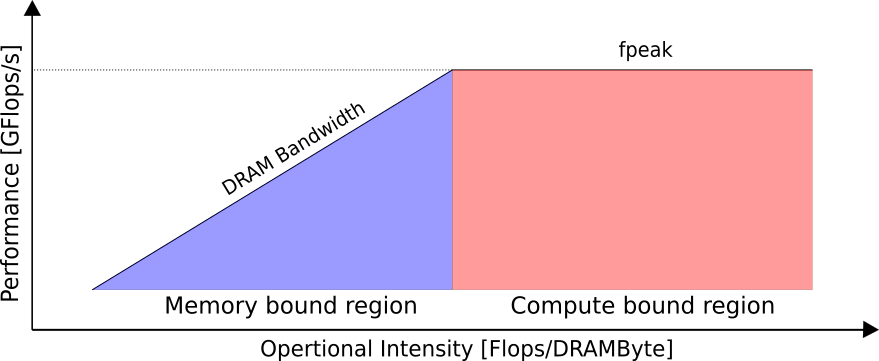
\includegraphics[width=\textwidth]{pictures/roofline_chart}
%%     \caption{ORM chart}
%%     \label{fig:roofline_chart}
%%   \end{minipage}
%%   \hfill
%%   \begin{minipage}[b]{0.49\textwidth}
%%     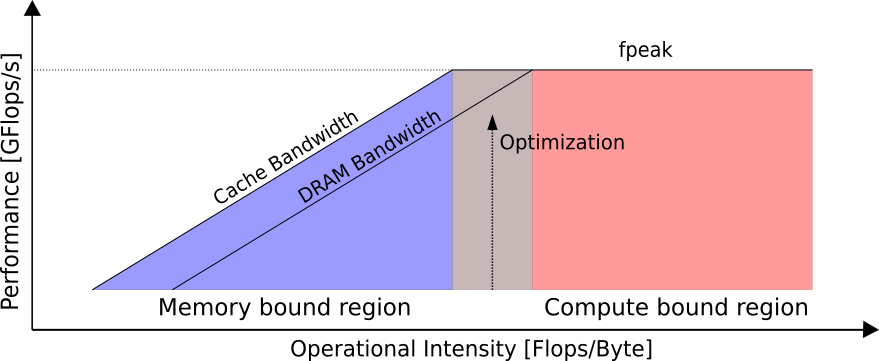
\includegraphics[width=\textwidth]{pictures/CARM_chart}
%%     \caption{CARM chart}
%%     \label{fig:CARM_chart}
%%   \end{minipage}
%%   \end{center}
%% \end{figure*}

In contrast, the CARM perceives the memory transfers from a consistent micro-architecture point of view, i.e., a core, where
the memory transactions are issued. As such, the CARM targets more contemporary systems where the PE encloses only compute units
and registers, while all other memory levels are separately and explicitly considered. For this purpose, the CARM includes several
memory lines in the same plot, each corresponding to the realistically achievable bandwidth of a specific memory level to the core,
i.e., cache levels and DRAM. When characterizing the applications, the CARM relies on the true "arithmetic intensity", i.e., the
ratio of performed compute operations (flops) over the total volume of requested data (in bytes) by taking into account the
complete memory hierarchy (i.e., caches and DRAM).
%% This model is plot on chart ~\ref{fig:CARM_chart} and shows whether an
%% application with a given arithmetic intensity is memory-bound or compute-bound if a straight vertical line hit a peak (FP) roof
%% or a bandwidth roof.

We base our methodology on the Cache Aware Roofline Model. 
As explained above, this model differs from the original one, and we think that the CARM is able to give more insight on
applications bottleneck analysis, and has more potential to be adapted to future memory designs. Moreover, the ORM has already a
dedicated tool~\cite{Lo2015} for a similar purpose as our, but our approach is totally different and target a more consistent and
concrete analysis.

\section{Locality-Aware Roofline Tool}\label{sec:contrib}
%+++++++++++++

Our main contribution consists in the development of the open-source tool named Locality Aware Roofline Tool (LART)\footnote{available at: https://github.com/NicolasDenoyelle/LARM-Locality-Aware-Roofline-Model-}, which
exploits hwloc topology detection to automatically build the Cache Aware Roofline Model (CARM).

\paragraph*{Main tool features.}

The proposed LART is composed of 3 main components, namely:
\begin{itemize}
\item A set of micro-benchmarks for automatic CARM construction on a given micro-architecture;
\item The library for counter-based extraction  of CARM metrics from a user application (i.e., the number of performed flops and
  transferred bytes, as well as the overall execution time);
\item A model visualization tool to present the architecture bounds and applications metrics extraction.
\end{itemize}

The first component consists in a program that automatically  builds the CARM for the specific processor micro-architecture where
the tool is run. By relying on a set of hwloc features, the proposed tool automatically detects the memory hierarchy and processor
compute capabilities, based on which specific micro-benchmarks are instantiated to deeply evaluate the bandwidth of each memory
level,  as well as the peak floating point (FP) performance according to the CARM methodology.
In addition, the proposed tools also permits to perform the CARM validation tests, by running a set of micro-benchmarks with
variable arithmetic intensity. 
The second component of the tool represents  a library with a set of API calls. These API calls are aimed at performing the
automatic CARM characterization of a given user application, by instrumenting the application source code.
To provide a wider cross-platform portability, this component relies on PAPI~\cite{mucci1999papi} features to collect all
necessary CARM metrics via hardware performance counters, i.e., to determine the application arithmetic intensity and performance.
The third component of the proposed tool is a command-line generating a visual plot of the CARM using platform analysis results. It
enables a user to plot applications metrics extracted with the library on the Roofline chart. The model validation and bandwidth
deviation can also be seen and provide a straightforward evaluation of the confidence one can grant to the model.

\paragraph*{Building the model from a hierarchical topology}

\begin{figure}
  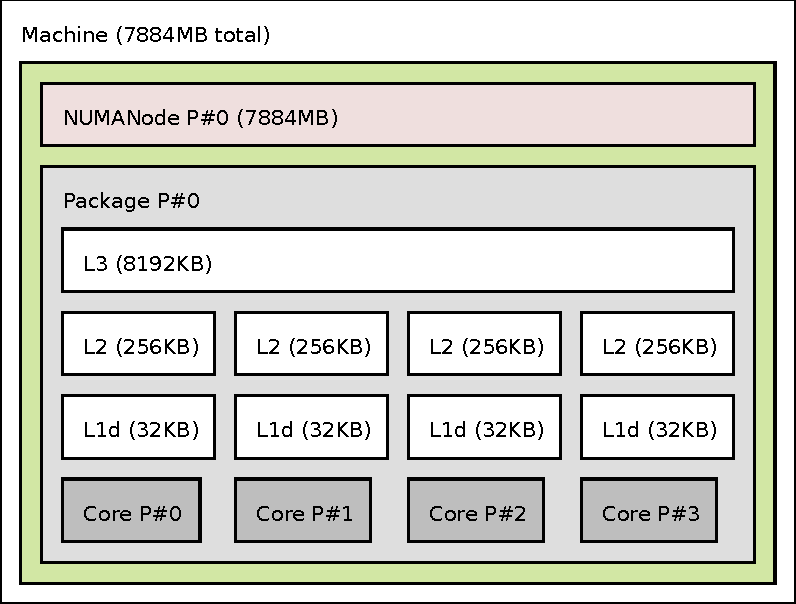
\includegraphics[width=.5\textwidth]{pictures/i7_3770k.pdf}
  \caption{Topology of Intel Ivy Bridge processor model i7 3770k as seen by hwloc}
  \label{fig:topology_adriana}
\end{figure}

Discovering all the computing and memory resources in a computing platform can be performed with tools such as
hwloc~\cite{goglin:hal-01330194}. Prior to hwloc,  the similar approaches were often less portable or they were not capable of
exposing as many details about cache sharing etc. The hwloc framework models the machine topology as a tree and suits particularly
well the caches structure.
As presented in Figure~\ref{fig:topology_adriana}, the view returned by the hwloc represents, express this structure with nested
boxes. Each core as a private stack of 2 caches, and every cores share the last level cache and the memory. This model where each
Core sees  the cache hierarchy as a cache stack of increasing size\footnote{
  The processors uses a cache replacement policy that removes old data from
  close caches in favor of more frequently used ones. The replacement policy move data from bottom caches to top caches. Since the
  space close to cores is thinner than the far space, the cache stack as seen by each core has an increasing size from bottom to
  top.
}, perfectly suits the way how the CARM perceives the memory hierarchy 
In addition, the hwloc library also allows a straightforward acquisition  of the cache and memory sizes via the  attributes of the
Core parent nodes. These parameters are further used in the proposed tool  in order to instantiate the appropriate micro-benchmarks
for different memory subsystem levels by using the state of the art technique (i.e buffer streaming of increasing sizes).

\paragraph*{Reaching the architecture upper-bounds}

Nowadays, processors usually implement a variety of vector operations, also named as Single Instruction Multiple Data (SIMD)
operations. Depending on the target micro-architecture,  the tool proposed herein is able to automatically detect the operation
type that allows to fully exploit the micro-architecture capabilities  (typically, the widest vector instructions). These
instructions refer to both compute operations and memory transactions, where the performance upper-bound of each involved unit is
expressed as a function of the registers size (i.e the number of floating point  elements it contains) and the achievable
throughput. By compiling the benchmarks on target architecture, we ensure that the largest vector size is used for the benchmarks
by interpreting the compiler macros. 

It is worth to emphasize that typically there are several types of memory/compute instructions on modern processors, lending
different pipelines and separate hardware units capable of performing different operations simultaneously. For instance, a core
may perform a multiplication (MUL) and an addition (ADD) on separate FPUs, which  can also be performed in parallel when there are
no  dependencies among them. Hence, a core can provide significantly higher  performance for the codes that fully interleave add
and MUL operations. This principle also applies to the memory subsystem, where several ports can be dedicated in modern processors
to simultaneously serve different number of load (LD) and store (ST) operations, e.g., 2 LD and 1 ST port in the newest Intel
micro-architectures. Hence, in order to exercise the full  compute and memory capabilities of the target architecture, the proposed
tool   relies on several types of usual operations to benchmark the platform and it picks by default the one used by the CARM, e.g.
for the Intel Ivy Bridge, it interleaves 2 LD and 1 ST instruction  when assessing the peak memory bandwidth, while 1 ADD and 1 MUL
are interleaved for peak FP performance. 

\paragraph*{CARM Experimental Results Reproduction}
\begin{figure*}
  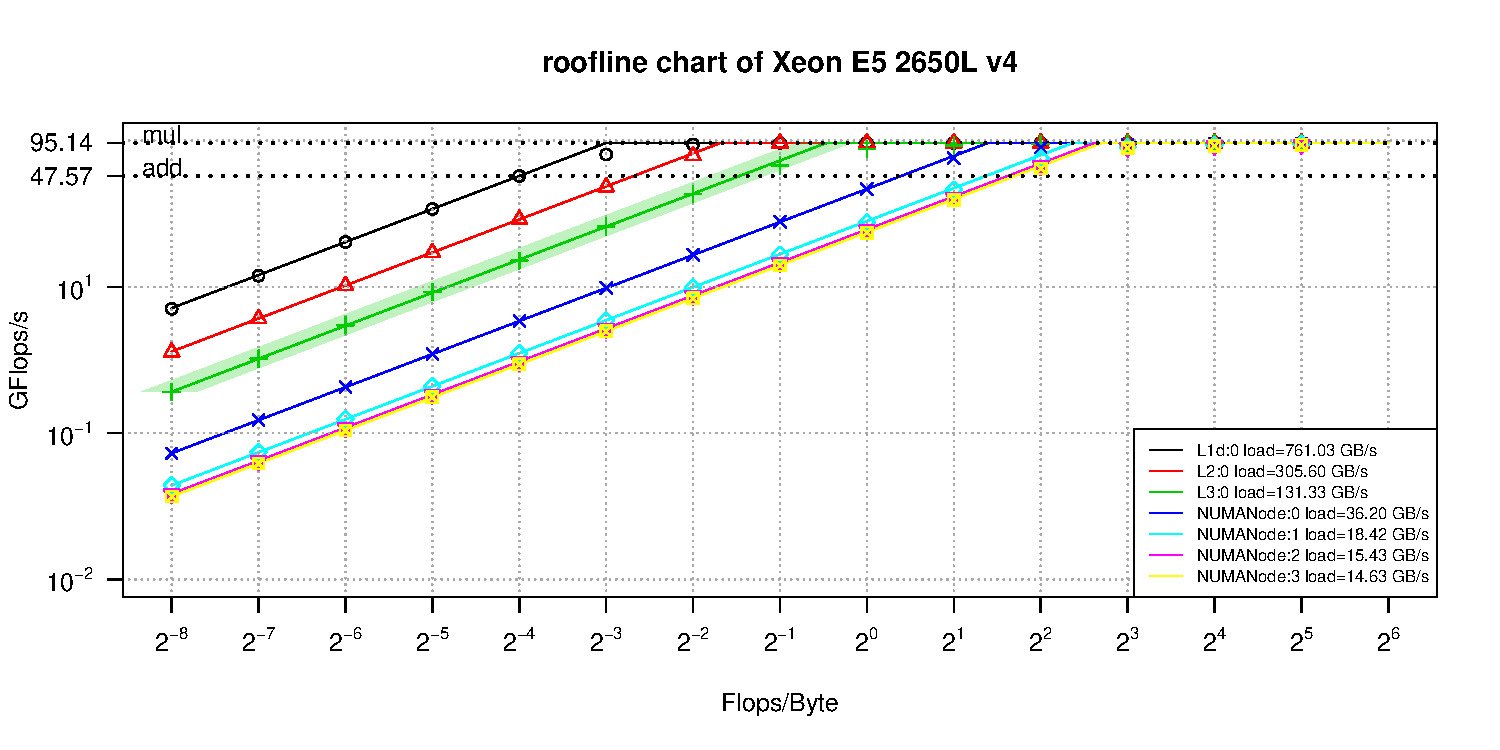
\includegraphics[width=\textwidth]{pictures/roofline_model}
  \caption{CARM on i7 3770k with LART tool.}
  \label{fig:LART_adriana}
\end{figure*}

Figure~\ref{fig:LART_adriana}, shows an output of the CARM plot generated by the herein proposed tool for an Intel i7
3770k (Ivy Bridge) processor, which topology is previously displayed in Figure~\ref{fig:topology_adriana}.
The black, red, green and blue oblique lines distinguish several regions of the attainable performance upper-bounds for AVX
instructions, which are limited by the bandwidth of different memory levels , i.e., L1, L2, L3 and DRAM, respectively.
The two horizontal lines represent the peak FP performance for multiplication/addition and multiplication with addition. 

It is worth to note that the proposed tool was capable of reaching the near-theoretical upper-bounds of the tested
micro-architecture both for the the L1 bandwidth and peak FP performance.  In particular, by relying on the CARM testing
methodology,  the throughput of 1.49 instructions per cycle (IPC) was achieved for the  L1 AVX accesses , while the achieved IPC of
1.98 for FP performances closely matches the theoretical throughput of AVX FP instructions when overlapping addition and
multiplication operations. 
The colored points matching the CARM lines represent the results of the validation benchmarks provided within the proposed tool,
i.e., a set of synthetic benchmarks tailored to hit the performance upper-bounds of the micro-architecture for different
arithmetic intensities.

On the bottom right corner, legend names shows first the memory subsystem, then the micro-operation type, here 2ld1st (i.e
interleaving of 2 LD and 1 ST) and finally the bandwidth value.
On the top right corner of the chart stands the legend for CARM metrics extracted from applications with our library. Those
application express different arithmetic intensity and are well suited to be explained with this model since they do not have
complicated branch and several arithmetic intensity statements. They represent application potential hot spot and come from well
known benchmarks named as HPCCG and STREAM. Deep performance evaluation of those applications is out of the scope of the paper, but
we here we show that the LART tool is capable of providing the facilities to do so.

\section{Conclusion and future work}\label{sec:conclusion}
%+++++++++++++++++++++++++++++++++++

On the path of extreme scale computing, computer systems complexity is increasing to address hardware and software constraints.
The CARM is able to aggregate this complexity and relying on hwloc topology detection capability, we implemented it in a robust
tool. It is capable of deep platform analysis and model validation with automatic detection of micro architecture and topology.
Additionally to avoiding non expert developers the pain of platform specific benchmarking, it provides a library to project and
visualize applications in the model. The performance we obtained on Intel Ivy Bridge micro-architecture matches near-theoretical
performances and proves the CARM methodology effectiveness.

In a close future, we plan to extend it to model heterogeneous memory systems and show it can be use to improve data spatial
locality when the current model is used to improve data temporal locality with cache usage optimization.

\bibliographystyle{plain}
\bibliography{references}

\end{document}
